\documentclass[tikz,border=3.14mm]{standalone}
\usetikzlibrary{decorations.pathmorphing}
\begin{document}
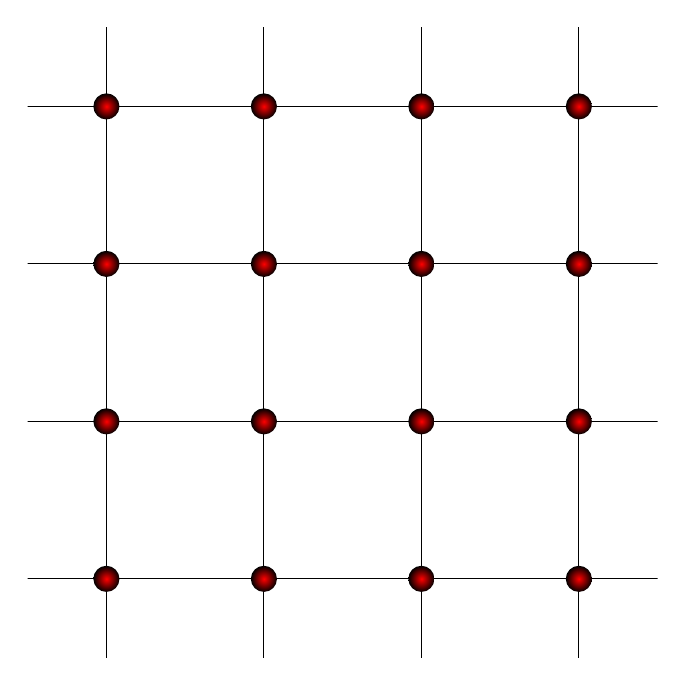
\begin{tikzpicture}
\clip (-1,-1) rectangle (7,7);
\foreach \X in {-2,0,...,10}
{\foreach \Y in {-2,0,...,10}
 {\draw[decorate,decoration={aspect=0.5,amplitude=1.5mm, segment
length=1.5mm}] (\X,\Y) -- ++(0,2) -- ++(2,0);
\node[circle,text=white,font=\sffamily\bfseries\large,inner
color=red,outer color=black] at (\X,\Y) {};}}
\end{tikzpicture}
\end{document}